\input ../SlidePreamble
\input ../preamble


\begin{document}

{\Huge


\centerline{\bf TTIC 31230, Fundamentals of Deep Learning}
\bigskip
\centerline{David McAllester, Winter 2020}

\vfill
\centerline{\bf Early Stopping, Shrinkage}
\vfill
\centerline{\bf Decoupled Shrinkage}
\vfill
\centerline{\bf Ensembles}
\vfill
\vfill

\slide{Training Data, Validation Data and Test Data}

Good performance on training data does not guarantee good performance on test data.

\vfill
An nth order polynomial can fit any n (pure noise) data points.

\slide{Loss Vs. Error Rate (or BLEU Score)}
While SGD is generally done on cross entropy loss, one often wants minimum classification error or BLEU Score (for translation).

\vfill
The term ``loss'' often refers to cross entropy loss as opposed to error rate.

\vfill
SGD optimizes loss because error is not differentiable.

\vfill
Later we will discuss attempts to directly optimize error.

\vfill
But training on loss is generally effective.


\slide{Early Stopping}

\centerline{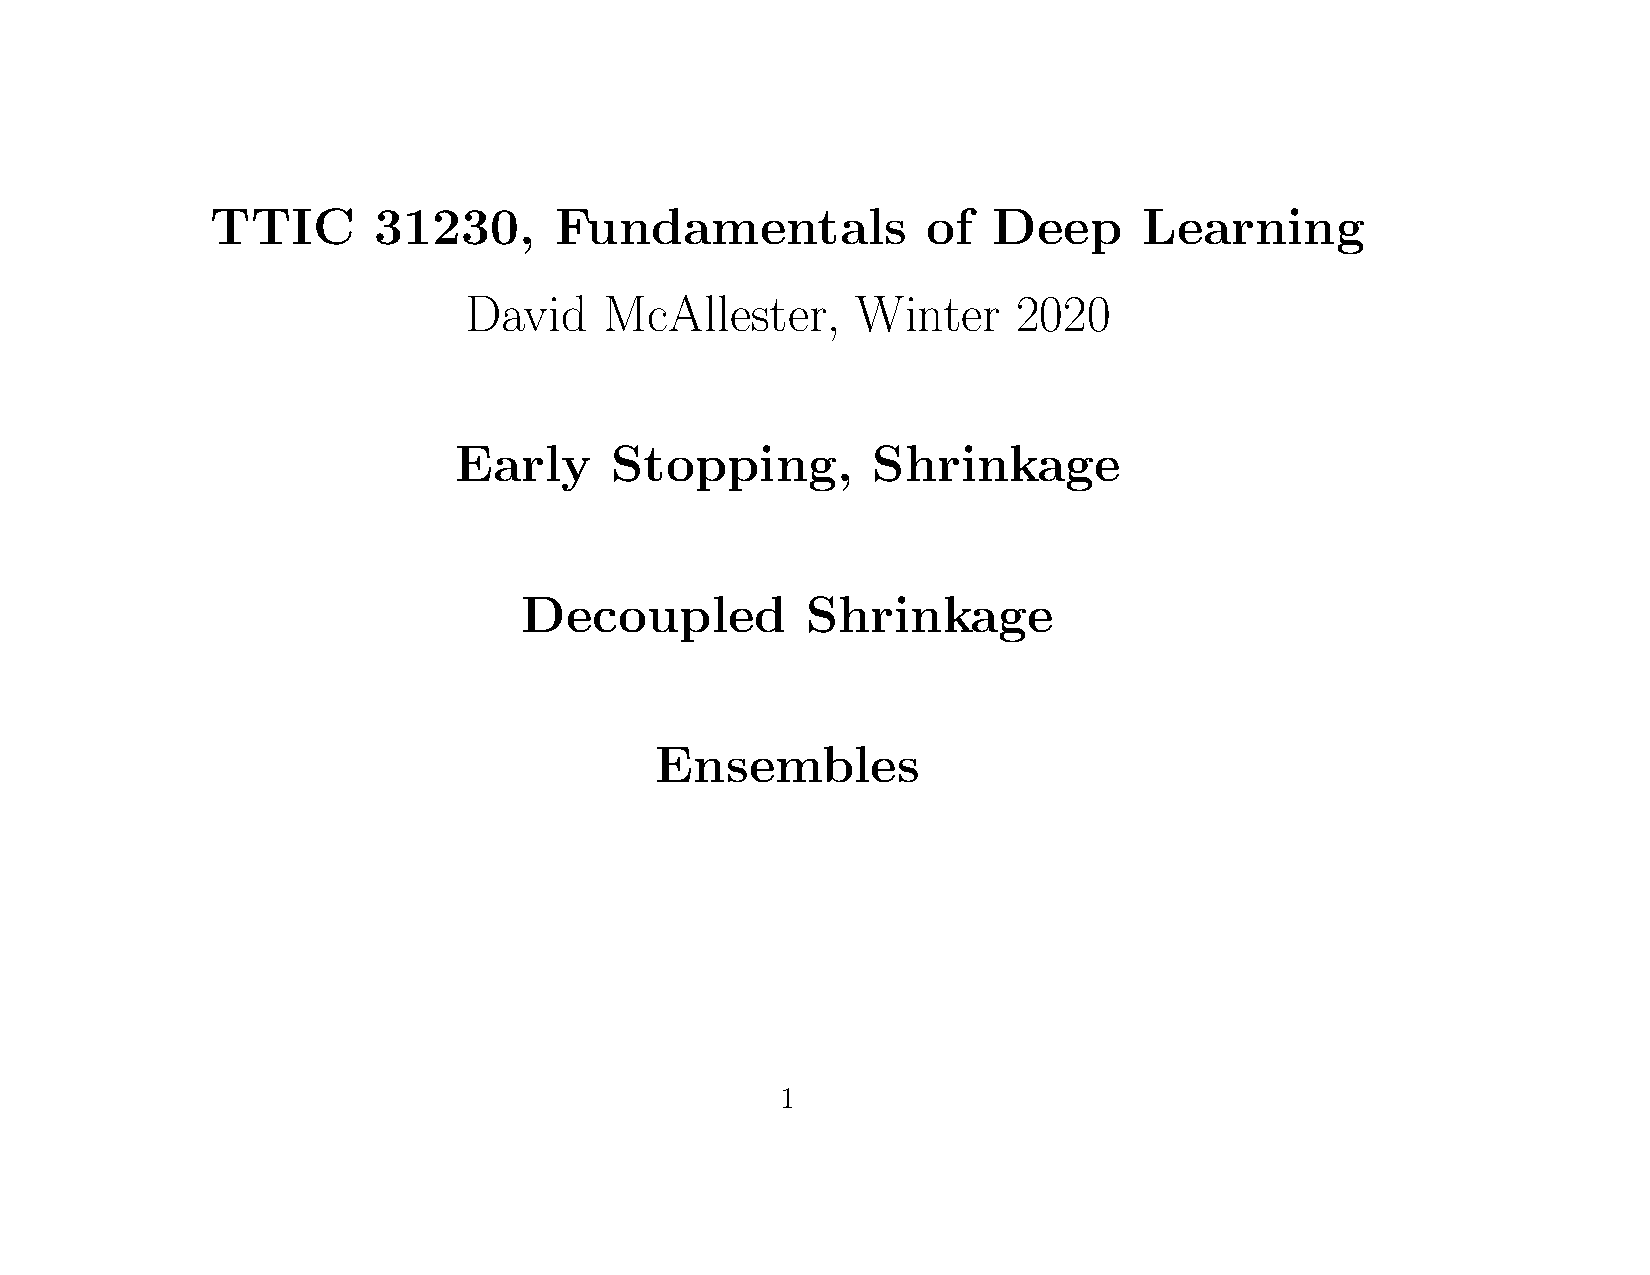
\includegraphics[height = 1.5in]{../images/Early}}

\centerline{\huge Claudia Perlich}

\vfill
During SGD one tracks validation loss and validation error.

\vfill
One stops training when the validation error stops improving.

\vfill
Empirically, loss reaches a minimum sooner than error.

\slide{Training Data, Validation Data and Test Data}

In general one designs algorithms and tunes hyper-parameters by training on training data and evaluating on validation data.

\vfill
But it is possible to over-fit the validation data (validation loss becomes smaller than test loss).

\vfill
Kaggle withholds test data until the final contest evaluation.


\slide{Over Confidence}

\centerline{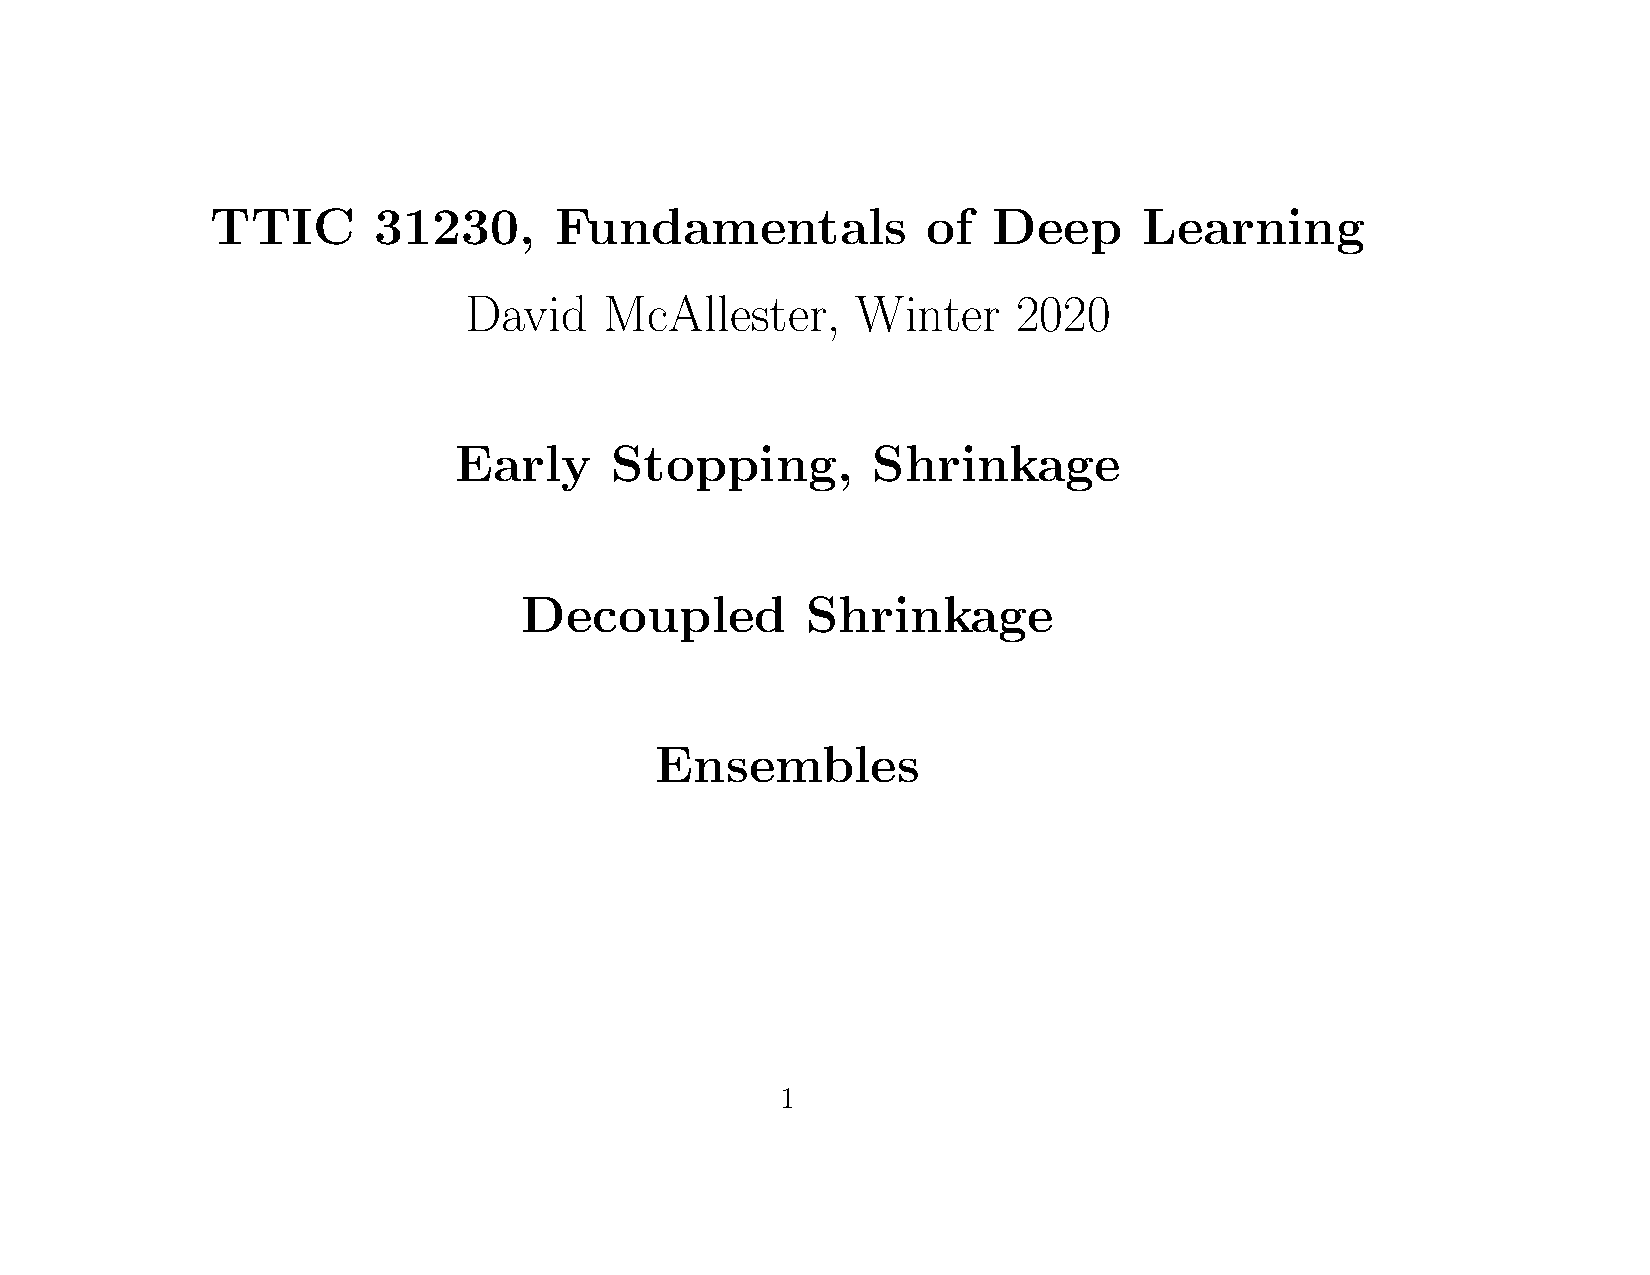
\includegraphics[height = 2in]{../images/Early}}

\vfill
Validation error is larger than training error when we stop.

\vfill
The model probabilities are tuned on training data statistics.

\vfill
The probabilities are tuned to an unrealistically low error rate and are therefore over-confident.

\vfill
This over-confidence occurs before the stopping point and damages validation loss (as opposed to validation error).

\slide{Regularization}

There is never harm in doing early stopping --- one should always do early stopping.

\vfill
Regularization is a modification to the training algorithm designed to reduce the training-validation gap and, in this way, improving overall performance.

\slide{Shrinkage: $L_2$ regularization}

Will first give a Bayesian derivation. We put a prior probability on $\Phi$ and maximize the posteriori probability (MAP).

\vfill
{\huge
\begin{eqnarray*}
\Phi^* & = & \argmax_\Phi\;p(\Phi | \tuple{x_1,y_1},\ldots,\tuple{x_n,y_n}) \\
\\
 & = & \argmax_\Phi\;p(\Phi,\;\tuple{x_1,y_1},\ldots,\tuple{x_n,y_n}) \\
 \\
  & = & \argmax_\Phi\;p(\Phi)P(\tuple{x_1,y_1},\ldots,\tuple{x_n,y_n}\;|\;\Phi) \\
 \\
 & = & \argmax_\Phi \; p(\Phi)\;\prod_i \pop(x_i)P_\Phi(y_i|x_i) \\
 \\
  & = & \argmax_\Phi \; p(\Phi)\;\prod_i P_\Phi(y_i|x_i)
 \end{eqnarray*}
}

\slide{Shrinkage: $L_2$ Regularization}

\begin{eqnarray*}
\Phi^*   & = & \argmax_\Phi \; p(\Phi)\;\prod_i P_\Phi(y_i|x_i) \\
\\
& = & \argmin_\Phi \sum_i - \ln P_\Phi(y_i|x_i) -\ln  p(\Phi)
\end{eqnarray*}

\vfill
We now take a Gaussian prior {\color{red} $$p(\Phi) \propto \exp\left(-\frac{||\Phi||^2}{2\sigma^2}\right)$$}

\slide{Shrinkage: $L_2$ Regularization}

\begin{eqnarray*}
\Phi^* & = & \argmin_\Phi \sum_{i = 1}^n - \ln P_\Phi(y_i|x_i) + \frac{||\Phi||^2}{2\sigma^2}  \\
\\
\\
& = & \argmin_\Phi \frac{1}{N} \left(\sum_{i = 1}^n - \ln P_\Phi(y_i|x_i) + \frac{||\Phi||^2}{2\sigma^2}\right)  \\
\\
\\
& = & \argmin_\Phi \left(E_{\tuple{x,y}\sim \mathrm{Train}}\;-\ln P_\Phi(y|x)\right) + \frac{1}{2N\sigma^2} ||\Phi||^2
\end{eqnarray*}

\slide{Shrinkage: $L_2$ Regularization}

\begin{eqnarray*}
  & & \nabla_\Phi \;E_{(x,y) \sim \mathrm{Train}}\;\left({\cal L}(\Phi,x,y) + \frac{||\Phi||^2}{2N\sigma^2}\right) \\
  \\
  \\
  & = & E_{(x,y) \sim \mathrm{Train}} \;\left(g(\Phi,x,y) + \frac{\Phi}{N\sigma^2}\right)
\end{eqnarray*}

\vfill
$$\Phi_{i+1} = \Phi_i - \eta\hat{g}_i  - \frac{\eta}{N\sigma^2}\Phi$$

\vfill
The last term in the update equation is called ``shrinkage''.

\slide{Decoupled Shrikgage}

$${\color{red} \Phi_{i+1}} = \Phi_i - \eta\hat{g} - \frac{\eta}{N\sigma^2}\Phi_i\;\;\;\; = {\color{red} \Phi_i - \eta\hat{g} - \gamma\Phi_i}$$

\vfill
Here $\gamma$ is the PyTorch shinkage parameter.

\vfill
To decouple $\gamma$ from other hyperparameters we can use

\vfill
{\color{red} $$\gamma = \frac{\eta}{N_{\mathrm{Train}}\sigma^2} = \frac{B\eta_0}{N_gN_{\mathrm{Train}}\sigma^2}$$}

\vfill
where $N_\mathrm{Train}$ is the number of training instances, $N_g$ is the decoupled momentum parameter, $\eta_0$ is the decoupled learning rate,
$B$ is the batch size, and $\sigma$ is the new decoupled shrinkage parameter.

\slide{Shrinkage meets Early Stopping}

Early stopping can limit $||\Phi||$.

\vfill
But early stopping more directly limits $||\Phi - \Phi_\mathrm{init}||$.

\vfill
It seems better to take the prior on $\Phi$ to be

\vfill
{\color{red} $$p(\Phi) \propto \exp\left(-\frac{||\Phi - \Phi_{\mathrm{init}}||^2}{2\sigma^2}\right)$$}

\vfill
giving

\vfill
$$\Phi_{t+1} = \Phi_t - \eta\hat{g} - \gamma(\Phi_t - \Phi_{\mathrm{init}})$$

\slide{$L_1$ Regularization and Sparse Weights}

$$p(\Phi) \propto e^{-\lambda ||\Phi||_1} \;\;\;\;\;\;\;\;||\Phi||_1 = \sum_i |\Phi_i|$$

$$\Phi^* = \argmin_\Phi \; \;\;\hat{\cal L}(\Phi) \;+ \; \;\frac{\lambda}{N_{\mathrm{Train}}}||\Phi||_1$$

\begin{eqnarray*}
  \Phi & \minuseq & \eta \nabla_\Phi \; \hat{\cal L}(\Phi) \\
  \Phi_i & \minuseq & (\eta\lambda/N_{\mathrm{Train}})\; \mathrm{sign}(\Phi_i) \;\;\;\;\;\;\mbox{(shrinkage)}
\end{eqnarray*}

\vfill
At equilibrium \hfill (sparsity is difficult to achieve with SGD)

$$\begin{array}{rcll}
\Phi_i &  = & 0  & \;\;\;\;\;\mbox{if} \;\left|\partial {\cal L} /\partial \Phi_i\right| <  \lambda/N_{\mathrm{Train}} \\
\partial {\cal L} /\partial \Phi_i & = &  -(\lambda/N_{\mathrm{Train}}) \mathrm{sign}(\Phi_i) &\;\;\;\;\; \mbox{otherwise}
\end{array}$$


\slide{Ensembles}

Train several models $\mathrm{Ens} = (\Phi_1,\;\ldots,\; \Phi_k)$ from different initializations and/or under different meta parameters.

\vfill
We define the ensemble model by
$$P_\mathrm{Ens}(y|x) = \frac{1}{k} \sum_{j=1}^k\; P_{\Phi_i}(y|x)$$

\vfill
Ensemble models almost always perform better than any single model.


\vfill
\slide{Ensembles Under Cross Entropy Loss}

For log loss we average the probabilities.

\vfill
$$P(y|x) = \frac{1}{k} \sum_i \;P_i(y|x)$$

\vfill
$- \log P$ is a convex function of $P$.  For any convex ${\cal L}(P)$ Jensen's inequality states that

$${\cal L}\left(\frac{1}{k} \sum_i P_i\right) \leq \frac{1}{k} \sum_i {\cal L}(P_i)$$

\vfill
This implies that the loss of the average model cannot be worse (can only be better) than the average loss of the models.

\vfill
\slide{Ensembles Under Cross Entropy Loss}

By Jensen:

$${\cal L}\left(\frac{1}{k} \sum_i P_i\right) \leq \frac{1}{k} \sum_i {\cal L}(P_i)$$

\vfill
However, in practice for each $i$ we have

$${\cal L}\left(\frac{1}{k} \sum_i P_i\right) \leq {\cal L}(P_i)$$

\slide{END}

}
\end{document}
